\setchapterstyle{kao}
\setchapterpreamble[u]{\margintoc}
\chapter{Introduction}
\labch{intro}

\section{The main ideas}
The book is in the following arrangement:
\begin{figure*}[h!]
	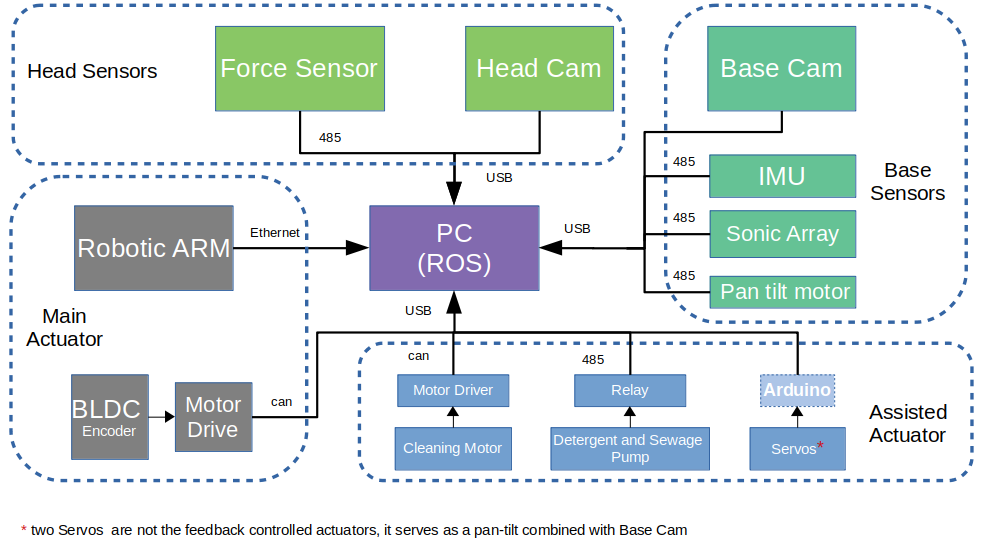
\includegraphics{01_hardware_all.png}
	\caption[Hardware structure]{Hardware structure of Window Cleaning Robot}
\end{figure*}


\begin{description}
	\item[style.sty] This package contains the specifications of page 
	layout, headers and footers, chapter headings, and the fonts used 
	throughout the document.
	\item[packages.sty] Loads additional packages to decorate the 
	writing with special contents (for instance, the \Package{listing} 
	package is loaded here as it is not required in every book). There 
	are also defined some useful commands to print the same words always 
	in the same way, \eg latin words in italics or \Package{packages} in 
	verbatim.
	\item[references.sty] Some useful commands to manage labeling and 
	referencing, again to ensure that the same elements are referenced 
	always in a consistent way.
	\item[environments.sty] Provides special environments, like boxes. 
	Both simple and complex environments are available; by complex we 
	mean that they are endowed with a counter, floating and can be put 
	in a special table of contents.\sidenote[-2mm][]{See 
	% \vrefch{34_MotorDriver} for some examples.
	}
	\item[theorems.sty] The style of mathematical environments. 
	Acutally, there are two such packages: one is for plain theorems, 
	\ie the theorems are printed in plain text; the other uses 
	\Package{mdframed} to draw a box around theorems. You can plug the 
	most appropriate style into its document.
\end{description}

